\section{Evaluation}


\begin{figure*}[tb]
    \centering
    \begin{subfigure}[b]{0.33\textwidth}
        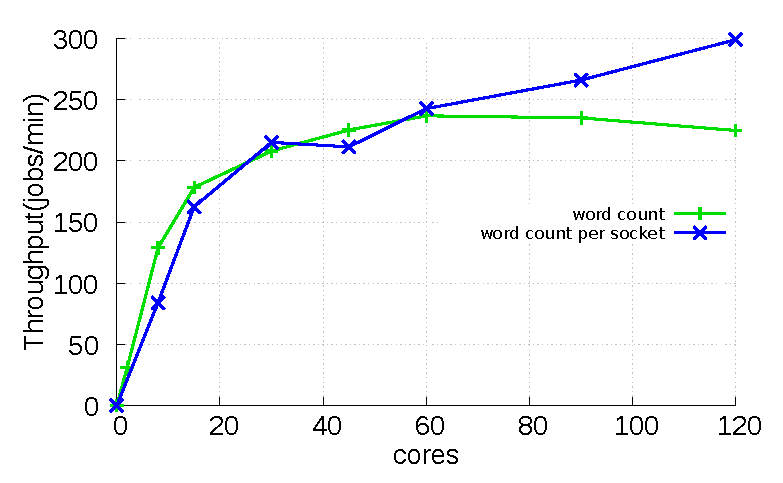
\includegraphics[width=2.2in]{graph/wc_docker.eps}
        \caption{Exim - 120core}
    \end{subfigure}%
    \begin{subfigure}[b]{0.33\textwidth}
        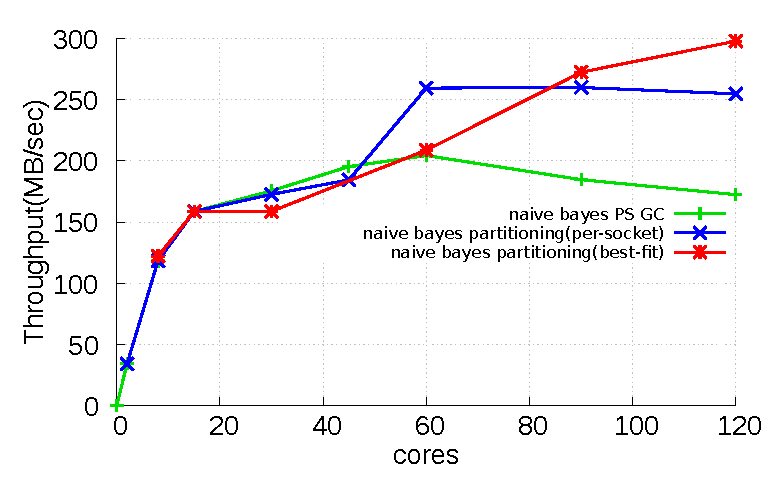
\includegraphics[width=2.2in]{graph/nb_docker.eps}
        \caption{Lmbench - 120core}
    \end{subfigure}%
    \begin{subfigure}[b]{0.33\textwidth}
        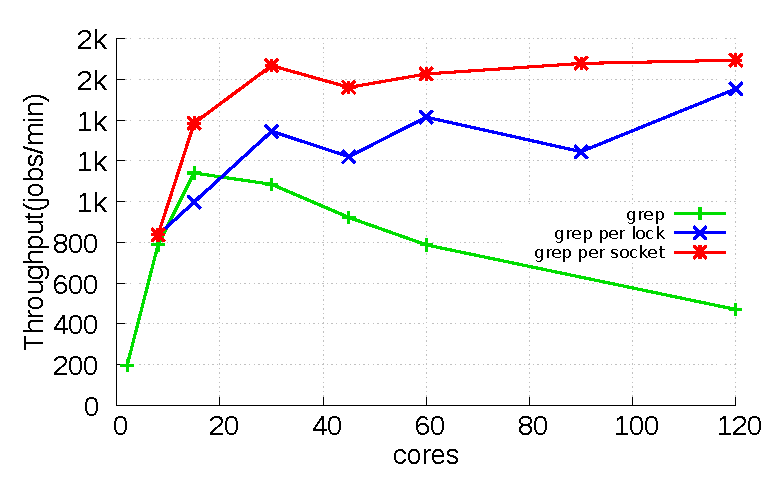
\includegraphics[width=2.2in]{graph/grep_docker.eps}
        \caption{AIM7 - 120core}
    \end{subfigure}
        \begin{subfigure}[b]{0.33\textwidth}
        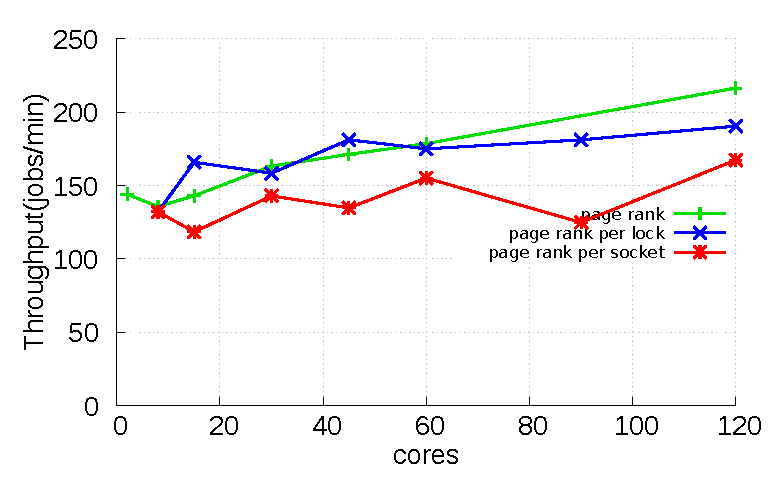
\includegraphics[width=2.2in]{graph/pagerank_docker.eps}
        \caption{Lmbench - 120core}
    \end{subfigure}%
        \begin{subfigure}[b]{0.33\textwidth}
        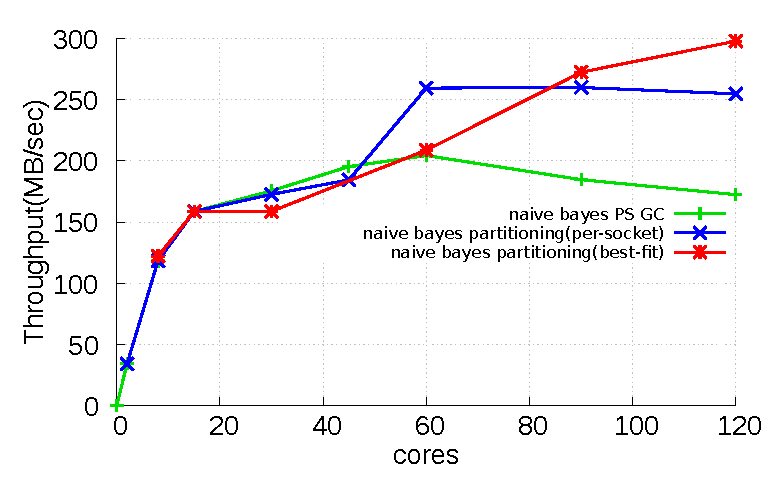
\includegraphics[width=2.2in]{graph/nb_docker.eps}
        \caption{Lmbench - 120core}
    \end{subfigure}%
    \begin{subfigure}[b]{0.33\textwidth}
        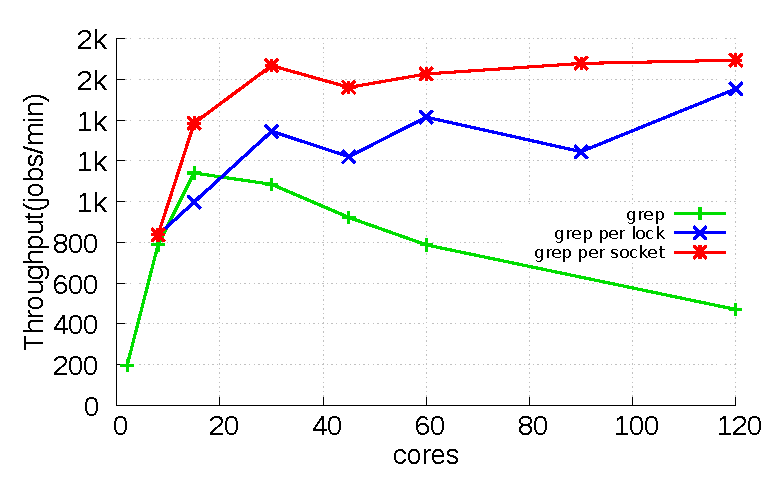
\includegraphics[width=2.2in]{graph/grep_docker.eps}
        \caption{AIM7 - 120core}
    \end{subfigure}
        \centering
    \caption{CPU utilization on 120 core.}
    \label{fig:utilization3}
\end{figure*}



\begin{figure*}[tb]
    \centering
    \begin{subfigure}[b]{0.25\textwidth}
        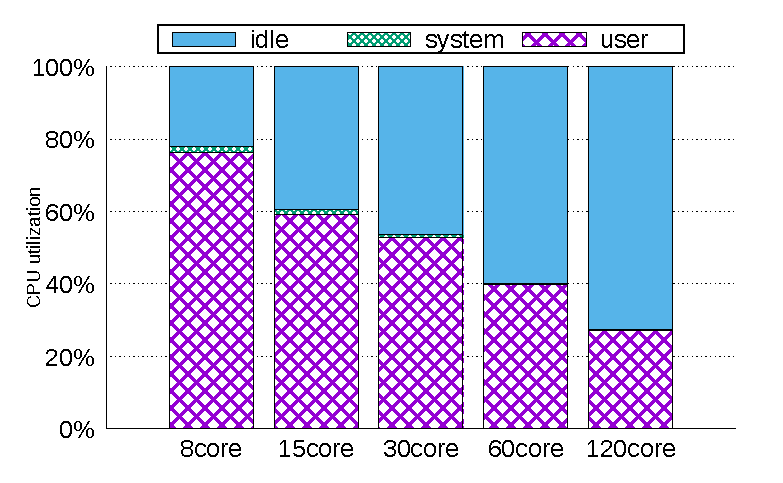
\includegraphics[width=1.8in]{graph/wc_cpuutils.eps}
        \caption{Word Count}
    \end{subfigure}%
    \begin{subfigure}[b]{0.25\textwidth}
        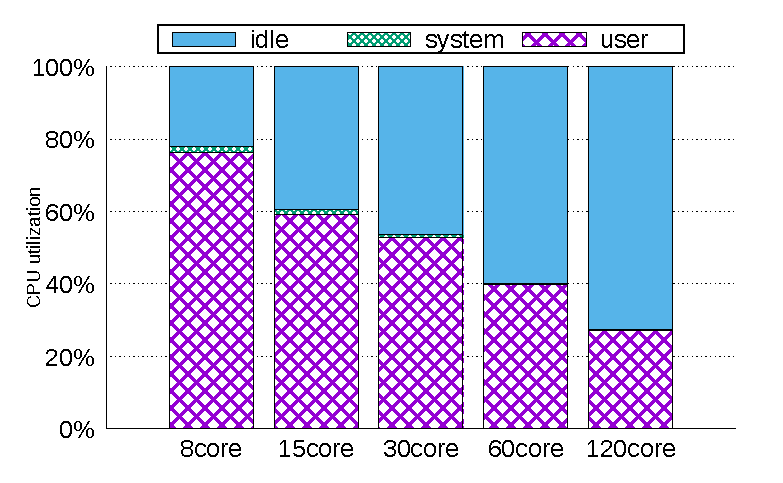
\includegraphics[width=1.8in]{graph/wc_cpuutils.eps}
        \caption{Naive Basian}
    \end{subfigure}%
    \begin{subfigure}[b]{0.25\textwidth}
        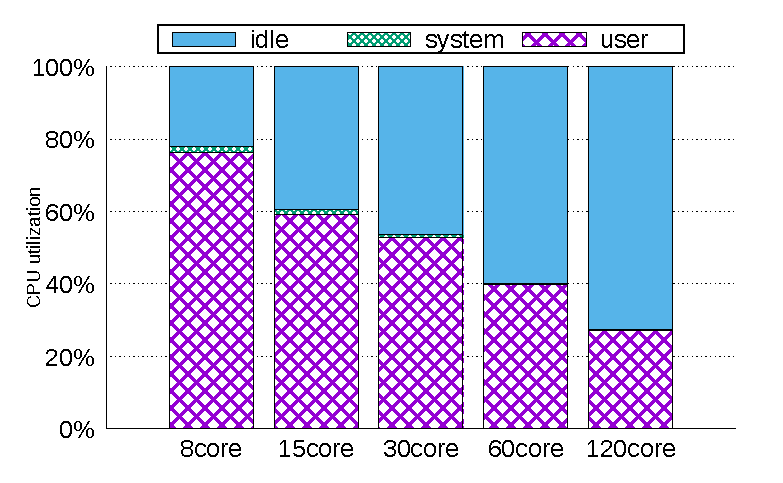
\includegraphics[width=1.8in]{graph/wc_cpuutils.eps}
        \caption{Grep}
    \end{subfigure}%
        \begin{subfigure}[b]{0.25\textwidth}
        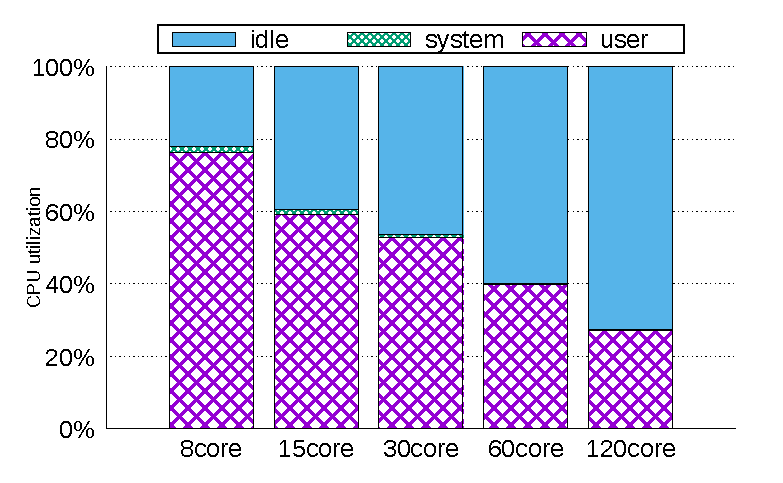
\includegraphics[width=1.8in]{graph/wc_cpuutils.eps}
        \caption{Pagerank}
    \end{subfigure}
        \centering
    \caption{CPU utilization on 120 core.}
    \label{fig:utilization2}
\end{figure*}


%$$$$$$$$$$$$$$$$$$$$$$$$$$$$$$$$$$$$$$$$$$$$$$$$$$$$$$$$$$$$$$$$$$$$$$$$$$$$$$$$
%Paragraph 1: 실험 환경 설명
%$$$$$$$$$$$$$$$$$$$$$$$$$$$$$$$$$$$$$$$$$$$$$$$$$$$$$$$$$$$$$$$$$$$$$$$$$$$$$$$$
\ifkor
이번 장에서는 스파크의 Scalalbility에 대해서 설명한다.
\else

\fi




%$$$$$$$$$$$$$$$$$$$$$$$$$$$$$$$$$$$$$$$$$$$$$$$$$$$$$$$$$$$$$$$$$$$$$$$$$$$$$$$$
%Paragraph 2: 비교 대상 설명
%$$$$$$$$$$$$$$$$$$$$$$$$$$$$$$$$$$$$$$$$$$$$$$$$$$$$$$$$$$$$$$$$$$$$$$$$$$$$$$$$
\ifkor
이번 장에서는 스파크의 Scalalbility에 대해서 설명한다.
\else

\fi




%$$$$$$$$$$$$$$$$$$$$$$$$$$$$$$$$$$$$$$$$$$$$$$$$$$$$$$$$$$$$$$$$$$$$$$$$$$$$$$$$
%Paragraph 2: A그룹에 대한 실험 결
%$$$$$$$$$$$$$$$$$$$$$$$$$$$$$$$$$$$$$$$$$$$$$$$$$$$$$$$$$$$$$$$$$$$$$$$$$$$$$$$$
\ifkor
이번 장에서는 스파크의 Scalalbility에 대해서 설명한다.
\else

\fi




%$$$$$$$$$$$$$$$$$$$$$$$$$$$$$$$$$$$$$$$$$$$$$$$$$$$$$$$$$$$$$$$$$$$$$$$$$$$$$$$$
%Paragraph 2: b그룹에 대한 실험 결
%$$$$$$$$$$$$$$$$$$$$$$$$$$$$$$$$$$$$$$$$$$$$$$$$$$$$$$$$$$$$$$$$$$$$$$$$$$$$$$$$
\ifkor
이번 장에서는 스파크의 Scalalbility에 대해서 설명한다.
\else

\fi



%$$$$$$$$$$$$$$$$$$$$$$$$$$$$$$$$$$$$$$$$$$$$$$$$$$$$$$$$$$$$$$$$$$$$$$$$$$$$$$$$
%Paragraph 2: CPU utilization에 대한 설명
%$$$$$$$$$$$$$$$$$$$$$$$$$$$$$$$$$$$$$$$$$$$$$$$$$$$$$$$$$$$$$$$$$$$$$$$$$$$$$$$$
\ifkor
이번 장에서는 스파크의 Scalalbility에 대해서 설명한다.
\else

\fi
